\subsection{User Study}
To further evaluate the effectiveness of $\avats$ from the the audience perspective, we conducted formal user studies to compare how users perform the urban exploration tasks with visualizations generated by whole dataset, \textit{random sampling} and $\avats$.


\begin{figure}[t]
	\centering
	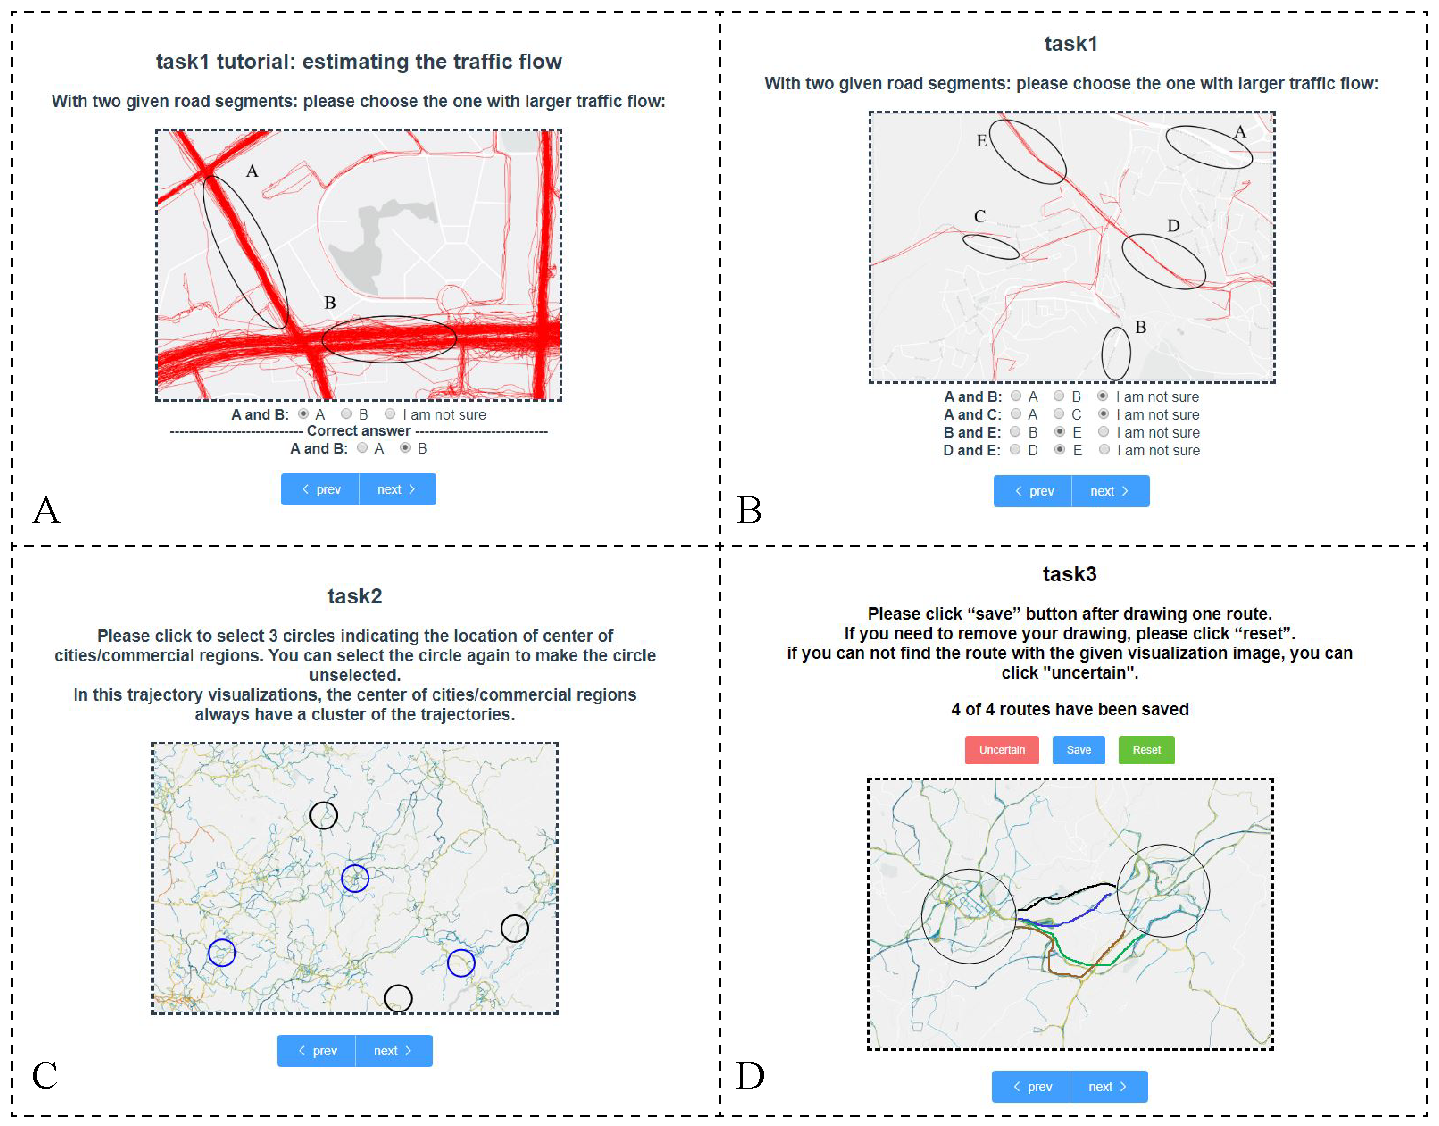
\includegraphics[width=0.48\textwidth]{pictures/user_study/interface.pdf}
	\vspace{-3mm}
	\caption{The interface of user study platform.}
	\vspace{-5mm}
	\label{fig:user_study}
\end{figure}

\subsubsection{Experiment setting}

\stitle{Participants and apparatus}
We recruit 100 participants (** females, ** males, aged 20 to **(mean=**, SD=**)) with normal vision or normal corrected vision. All of these participants have the background of computer science. 
The study system is a web-based platform which has the size-fixed interface and the participants perform the user study on their own  computers. The system interface is shown as Figure~\ref{fig:user_study}. Considering the unfairness caused by the screen size, we recommend all participants to set the resolution of the screen as 1980 * 1080 before the experiment. All images displayed on the interface have the same size of(AA*BB).  

\stitle{Tasks}
All participants needed to perform three types of tasks(shown as Figure~\ref{fig:user_study}(B,C,D)):
\setlist{nolistsep}
\begin{itemize}[noitemsep]
	\item \textbf{T1. Traffic flow estimation.} 
	The participants are asked to select the road segment with higher traffic flow from two candidates.
	A road with larger traffic flow has more trajectories in the dataset passing through the road segment, thus lead to a denser and broader trajectory brunch in the visualization.  In the trajectory visualization with color encoding, such kind of pattern can also be highlighted by a concentration of trajectories with warm color.
	\item \textbf{T2. City/commercial region center identification.} The participants need to identify the centers of the cities or commercial regions through the trajectory visualization. The city or commercial region centers always have more passing trajectories from different directions than the surrounding regions which results in the  \UC{start-shape} cluster of trajectories in the visualization.
	\item \textbf{T3. Reachable route inspection.} The reachable routes indicate the routes connecting two regions, these routes must have the passing trajectories. The participants were asked to inspect the reachable routes between the two regions by drawing lines. 
	%\item \textbf{T4. Visual similarity comparison.} With a given visualization generated by full dataset as ground truth, the participants were asked to rank a set of visualizations according to the similarity to the ground truth. 
\end{itemize}

\stitle{Data generation}
We used the taxi trajectory dataset of Porto and Shenzhen for the user study. The testing data for each type of tasks were generated as follows:

\textbf{Tasks of T1.} We selected several visualization views which contain clear road structures. Then the number of trajectories passing through each road segment was counted as the traffic flow of this road segment. In the tasks of T1, two road segments in a view are given randomly, and the users needed to select the one with higher traffic flow.  

\textbf{Tasks of T2.} We randomly chose several visualization views which contain city/commercial regions and labeled the locations of each city/commercial region center on the visualization as the correct locations first.  Then we randomly generated locations and remove the locations close to the correct locations, the remaining locations are the error locations. In each task of T2, with a given visualization, the same number of correct and wrong locations will be randomly selected and the participants were asked to select the locations indicating the city/commercial region centers. 

\textbf{Tasks of T3.} We randomly chose several visualization views which contain two or more city/commercial regions, which will be marked by circles. In each task of T3, an visualization view and two regions will be selected randomly.
%In the tasks of T3, the users were asked to draw the reachable routes between the two selected regions. 

%\textbf{Tasks of T4.} With a given center location and zoom scale, we generated the visualizations by using whole dataset, uniform random sampling and $\avats$ with different parameters. Using visualization generated by whole dataset as ground truth, users were required to score the other visualizations according to the similarity to the ground truth.  

\stitle{Procedure}
The user study began with the introduction which introduces the motivation, tasks and visual encoding. Then the following sessions are divided into three blocks according to the task types. Each block starts with a task tutorial, in which the participants could perform several demo tasks, thus familiarizing themselves with the interface, interaction and tasks. For example, Figure~\ref{fig:user_study}(A) shows the demo task of T1, in which the users can check the correct answer after clicking the ``check'' button. 
In each task of T1, with a given visualization, multiple road segment will be identified by ellipses(shown as~\ref{fig:user_study}(B)). Several road segment pairs are listed under the visualizations. The participants were asked to choose the one with larger traffic flow by clicking the radio box. They can also choose ``I am not sure'' if they cannot decided the answer. 
In each task of T2, a visualization view is given and several regions are marked by circles(as shown by Figure~\ref{fig:user_study}(C)). The users needed select the regions which could be city/commercial centers by click the corresponding circles. In each task, the number of correct regions are given. 
In each task of T3, with a visualization view and two circles(shown as Figure~\ref{fig:user_study}(D)), the users needed to draw several most representative reachable routes to connect the two circular regions. The number of the reachable routes is given.  
%The user study began with the introduction, in which the motivation, tasks and visual encoding were introduced. The following sessions are divided into three blocks according to the task types. Each block starts with a task tutorial, in which the participants could perform several demo tasks and were free to ask questions, thus familiarizing themselves with the interface, interaction and tasks.
%Then the users were asked to finish five normal tasks. During this procedure, both the answer and the time usage are recorded.
%After all the tasks were finished, the participants would fill a questionnaire about their comments. 

\subsubsection{Results}

\stitle{Accuracy}

\stitle{Time usage}

\stitle{User feedback}